\section{Particle analysis}
\label{sec:particle}

%``stagnation'' G and P stop moving

%``leader stagnation'' G stop moving

%``general unimodal'' (ISS of posotion update $ \rightarrow $ parameter values: consistent with past results )
%\begin{itemize}
%\item [theorem] in stagnation, inputs are bounded $ \rightarrow $ $ x(k+1) $ is bounded \\
%(like previous results) \\
%$  x^{*} = x^{G} = x^{P} $ \\
%$  \hat{x^{*}} = x^{G} \not = x^{P} $
%\item in unimodal case (smooth?)  \\
%1) (Lemma ?) when $ x^{G} = x^{*} $, input update is ISS \\
%2) (Lemma 1) when $ x^{G} = x^{*} $, ISS position update parameters, then particle is ISS \\
%2) (theorem ?) ..... then $ x \rightarrow x^{G} $ \\
%3) (Lemma 2) if $ x^{G} \not = x^{*} $ surely not stop at $ x^{G} $ \\
%4) (theorem 3) almost surly $ | x^{*} - x(k) | < \epsilon $ \\
%Lemma ? if unimodal then input update is ISS \\
%Needed: lemma 2 (?), Bound covers some non-zero set of points $ X $, where $ \forall x \in X, f(x) > f(x^{G}) $ \\
%Use def of "almost surly" - coin example \\
%maybe use fig. 7 with transition prob > 0 (Markov process) 
%\item in multimodal case \\
%lemma 3 \\
%corollary 2 $ \rightarrow $ theorem \\
%(theorem) Add the case for $ x^{*} $ outside of bound formed by $ x^{G} $ and $ x^{P} $ in this case (prob of finding $ x^{*} $) = 0.
%\end{itemize}

In one global-best stagnation, the global best is unchanged.
Thus we denote the global best as a constant $ x^{G} $ in one global-best stagnation.
In this case, the movement of any particle in the swarm is not influenced by any other particles till any particle in the swarm finds a better solution.
The particle with the leader role might deviate from $ x^{G}(k) $ due to the velocity inertia.
But it will gradually converge to $ x^{G}(k) $ by Equation \eqref{eq:up_vel:leader}.
The particle with the follower role is hard to evaluate because there are effects from both the personal best and the global best.
In one global-best stagnation, we are interested with 
\begin{itemize}
\item whether the particle converges to the global best;
\item and the probability that the particle find a new global best.
\end{itemize}

One way of measuring how the particle converges to the global best, we let $ x^{G} $ be the reference position $ x^{R} $ and get \eqref{eq:rel_gb}.

\begin{equation}
\label{eq:rel_gb}
\begin{aligned}
\begin{bmatrix}
v(k+1) \\
x(k+1) - x^{G}
\end{bmatrix}
 = A(k) 
\begin{bmatrix}
v(k) \\
x(k) - x^{G}
\end{bmatrix}
+ B(k) 
\begin{bmatrix}
0 \\
x^{P}(k) - x^{G}
\end{bmatrix}
\end{aligned}
\end{equation}

Apparently if the movement bounded region does not cover the optimal, the particle will not be able to get into the optimal position.
We have property \ref{prop:particle:nonoptimal}.

\begin{myprop}
\label{prop:particle:nonoptimal}
Whether a particle can reach the optimal is impacted by the boundary of its movement.
\end{myprop}

\begin{figure}[tbph]
\centering
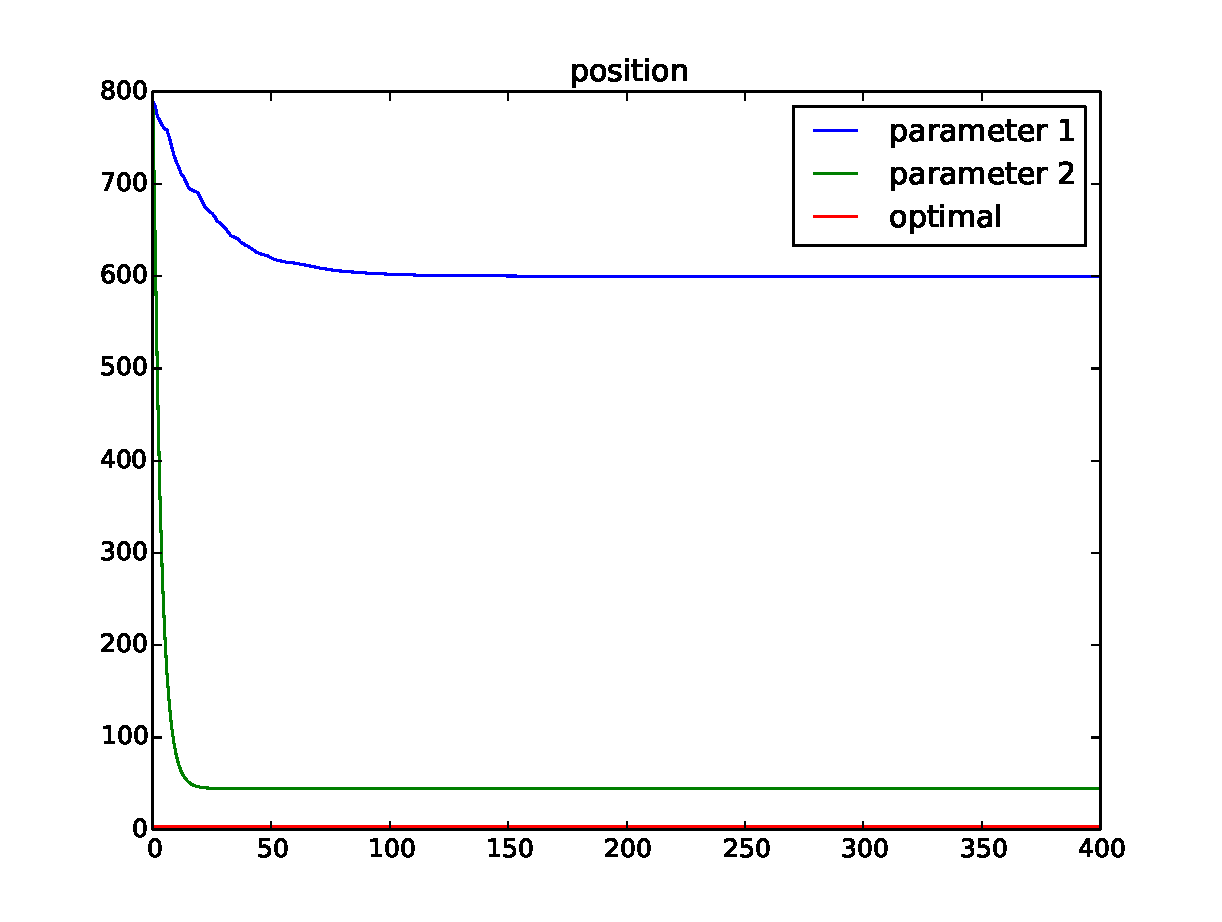
\includegraphics[width=0.7\linewidth]{./simfig/bound/bound_position}
\caption{The convergence to the optimal of particles with different parameters.}
\label{fig:bound_position}
\end{figure}

By Theorem \ref{thm:state_bound}, we know that the size of the boundary are determined by both  $ | x^{P} - x^{G} | $ and the parameters.
Figure \ref{fig:bound_position} gives an example on the boundary impacting the moving toward the optimal.
Parameter 1 is $ \chi = 0.3, \phi^{P} = 0.2, \phi^{G} = 0.2 $ and parameter 2 is $ \chi = 0.72984, \phi^{P} = 2.05, \phi^{G} = 2.05 $.
As a result, parameter 1 makes a smaller movement boundary, which prevents the particle reaching the optimal.

\subsection{Stagnation}

In stagnation, both the personal best and the global best are not updated, which can be denoted as constant, $ x^{P} $ and $ x^{G} $ respectively.
By Theorem \ref{thm:state_bound}, we know that $ \lVert x(k) - x^{G} \rVert $ indicates the distance from position $ x(k) $ to the global best, which depends on  $ \lVert x^{P} - x^{G} \rVert $.
Thus we have Theorem \ref{thm:stagnation_bound}.

\begin{mythm}
\label{thm:stagnation_bound}
\begin{equation}
\label{eq:stagnation_bound}
| x(k) - x^{G} | \leq \gamma ( | x^{P}(k) - x^{G} | ), 
\end{equation}
Particularly, when $ x^{P} $ is constant,
$  | x(k) - x^{G} | \leq \gamma ( | x^{P} - x^{G} | ). $
$ \gamma () $ is a boundary function.
\end{mythm}

Theorem \ref{thm:stagnation_bound} indicates how the movement of the particle is bounded by the distance between the global best and the personal best.
The result of the stagnation is not enough to evaluate the convergence of the entire optimal search.
A stagnation is a sub-section of a global-best stagnation.
A sequence of global-best stagnations consist of the procedure of the PSO.
We need the results of the global-best stagnation for the convergence analysis.
We look at two categories of fitness distribution, unimodal and multi-modal respectively in following two subsections.

\subsection{Unimodal fitness distribution}

Unimodal is one of the most typical fitness distributions.
It provides a partial monotonic form.
Any form of fitness distribution can be approximated as a combination of unimodalities.
In most of the cases, the particles finally convergence towards one unimodal of a fitness distribution.
Unimodal fitness distribution is a typical and bare case to analyze.
In a unimodal fitness distribution, there are two type of cases, $ x^{G} = x^{*} $ and $ x^{G} \neq x^{*} $.

\subsubsection{$ x^{G} = x^{*} $}

When $ x^{G} = x^{*} $, it means that the global best is already the optimal solution.
There is no chance for a particle to find a better.
By Theorem \ref{thm:unimodal:particle:converge}, we know that the particle should gradually converge to the global best if the position-update component is input-to-state stable.
The fitness distribution determines the property of the personal best update component.
We have the condition of the fitness distribution that makes the personal best update component input-to-state stable.
It is given in Lemma \ref{lem:unimodal:particle:input_iss}.

\begin{mylem}
\label{lem:unimodal:particle:input_iss}
If $ f(x^{*}) - \alpha_{2} ( |x| ) <  f(x) < f(x^{*}) - \alpha_{1} ( |x| ) $, when $ x^{G} = x^{*} $, the personal best update component is input-to-state stable.
$ \alpha_{1} () $ and $ \alpha_{2} () $ are $ K_{\infty} $-function.
\begin{proof}
Let $ V(x^{P}(k)) = f(x^{G}) - f(x^{P}(k)) $.
Because we have
$ \alpha_{1} ( |x^{P}(k)| ) \leq V( x^{P}(k) ) \leq \alpha_{2} ( |x^{P}(k)| )  $.
We have $ V ( x^{P}(k) ) $ satisfying condition 1 of the ISS-Lyapunov function definition.

We also have
\begin{equation}
\begin{aligned}
& V(x^{P}(k+1)) - V(x^{P}(k)) \\
= & f(x^{P} (k)) - f(x^{P} (k+1)) \\
= & f(x^{P}(k)) - f( \arg \max_{ \{ x^{P}(k), x(k+1)  \} } f(x) )  \\
= & 
\left\{\begin{matrix}
0  & \mbox{if } f(x(k+1)) \leq f(x^{P}(k)) \\ 
f(x^{P}(k)) - f(x(k+1)) & \mbox{if } f(x(k+1)) > f(x^{P}(k))
\end{matrix}\right. \\
\leq & 
\left\{\begin{matrix}
f(x^{P}(k)) - f(x(k+1))  & \mbox{if } f(x(k+1)) \leq f(x^{P}(k)) \\ 
f(x^{P}(k)) - f(x(k+1)) & \mbox{if } f(x(k+1)) > f(x^{P}(k))
\end{matrix}\right. \\
\leq & f(x^{P}(k)) - f(x(k+1)) \\
\leq & - V(x^{P}(k)) + V(x(k+1)) \\
\leq & - \alpha_{1} ( | x^{P}(k) | ) + \alpha_{2} ( | x(k+1) | ).
\end{aligned}
\end{equation} 
We have that $ \alpha_{1} () $ is $ K_{\infty} $-function and $ \alpha_{2} () $ is $ K $-function.
Thus the condition 2 of the ISS-Lyapunov function definition is also satisfied.
$ V(x) $ is an ISS-Lyapunov function.
By Lemma 3.5 in \cite{Jiang2001857}, in this case, the personal best update component is input-to-state stable.
\end{proof}
\end{mylem}

When both two components of a particle are input-to-state stable, we can have the condition that the particle is input-to-state stable in Lemma \ref{lem:unimodal:particle:iss}.

\begin{mylem}
\label{lem:unimodal:particle:iss}
When the position update component is input-to-state stable,
$ | x (k) | \leq \max \{ \beta_{1} (| x(0) |, k ), \gamma^{P}_{1} ( | x^{P} (k) | ), \gamma^{G}_{1} ( | x^{G} | ) \} $,
and the personal best update component is input-to-state stable,
$ | x^{P} (k) | \leq \max \{ \beta_{2} (| x^{P}(0) |, k ), \gamma_{2} ( | x^{P} (k) | ) $,
if $ \gamma^{P}_{1} \circ \gamma_{2} (s)  < s $, the feedback model of a particle is input-to-state stable.
\begin{proof}
By Theorem 2 in \cite{Jiang2001857}, we can directly have Lemma \ref{lem:unimodal:particle:iss}.
\end{proof}
\end{mylem}

We can have the condition that the particle converge to the optimal $ x^{*} $ in Theorem \ref{thm:unimodal:particle:garuantee_converge}.
The unimodal fitness distribution is one of the cases that satisfy $ f(x^{*}) - \alpha_{2} ( |x| ) \leq  f(x) \leq f(x^{*}) - \alpha_{1} ( |x| ) $.

\begin{mythm}
\label{thm:unimodal:particle:garuantee_converge}
When $ x^{G} = x^{*} $,  if $ f(x^{*}) - \alpha_{2} ( |x| ) \leq  f(x) \leq f(x^{*}) - \alpha_{1} ( |x| ) $ and $ \gamma_{1} \circ \gamma_{2} (s)  < s $, the particle will converge to $ x^{*} $ if the position-update component of the particle is input-to-state stable.
$ \gamma_{1} () $ is the gain of the position update component and $ \gamma_{2} () $ is the gain of the input update component.
\begin{proof}
By Lemma \ref{lem:unimodal:particle:iss}, we have the feedback model of the particle is input-to-state stable.
Because $ x^{G} = x^{*} $, the input to the cascade model of the particle is zero, $ | x^{G} - x^{*} | = 0 $.
By the property of the input-to-state stability, $ | x(k) - x^{*} | $ will converge to zero, which means that the particle will converge to $ x^{*} $.
\end{proof}
\end{mythm}

Theorem \ref{thm:unimodal:particle:garuantee_converge} shows the condition that the convergence could be guaranteed.
If we consider the stochastic terms in the position update component, $ \gamma_{1} \circ \gamma_{2} (s)  < s $ is not easy to guarantee.
Because $ \phi^{P} u^{P} (k) $ and $  \phi^{G} u^{G} (k)  $ are randomly sampled at each iteration.
However, the stochastic terms contribute to the almost surely convergence.
We can have Theorem \ref{thm:unimodal:particle:converge}.

\begin{mythm}
\label{thm:unimodal:particle:converge}
In a unimodal case, when $ x^{G} = x^{*} $, the particle will almost surely converge to $ x^{*} $ if the position-update component of the particle is input-to-state stable.
\begin{proof}
The convergence of the particle depends on the convergence of the personal best.
In this case, given the personal best $ x^{P} $, the solution space $ \Omega = A \cup B \land A \cap B = \phi $, in which 
$ A = \{ x | f(x) > f(x^{P}) \} $ and $ B = \{ x | f(x) \leq f(x^{P}) \} $.
As long as the particle gets into the set $ A $, the size of the set $ A $ decreases.
When $ A = \phi $, $ x^{P} = x^{G} = x^{*} $.
Set $ A $ should either be kept unchanged or be decreased.
The probability that set $ A $ is decreased should always be bigger than zero.
Thus, the size of $ A $ will almost surely converge to zero.
It means that the personal best will almost surely converge to the global best, which leads to that the particle almost surely converge to $ x^{G}  = x^{*} $.

\begin{figure}[tbph]
\centering
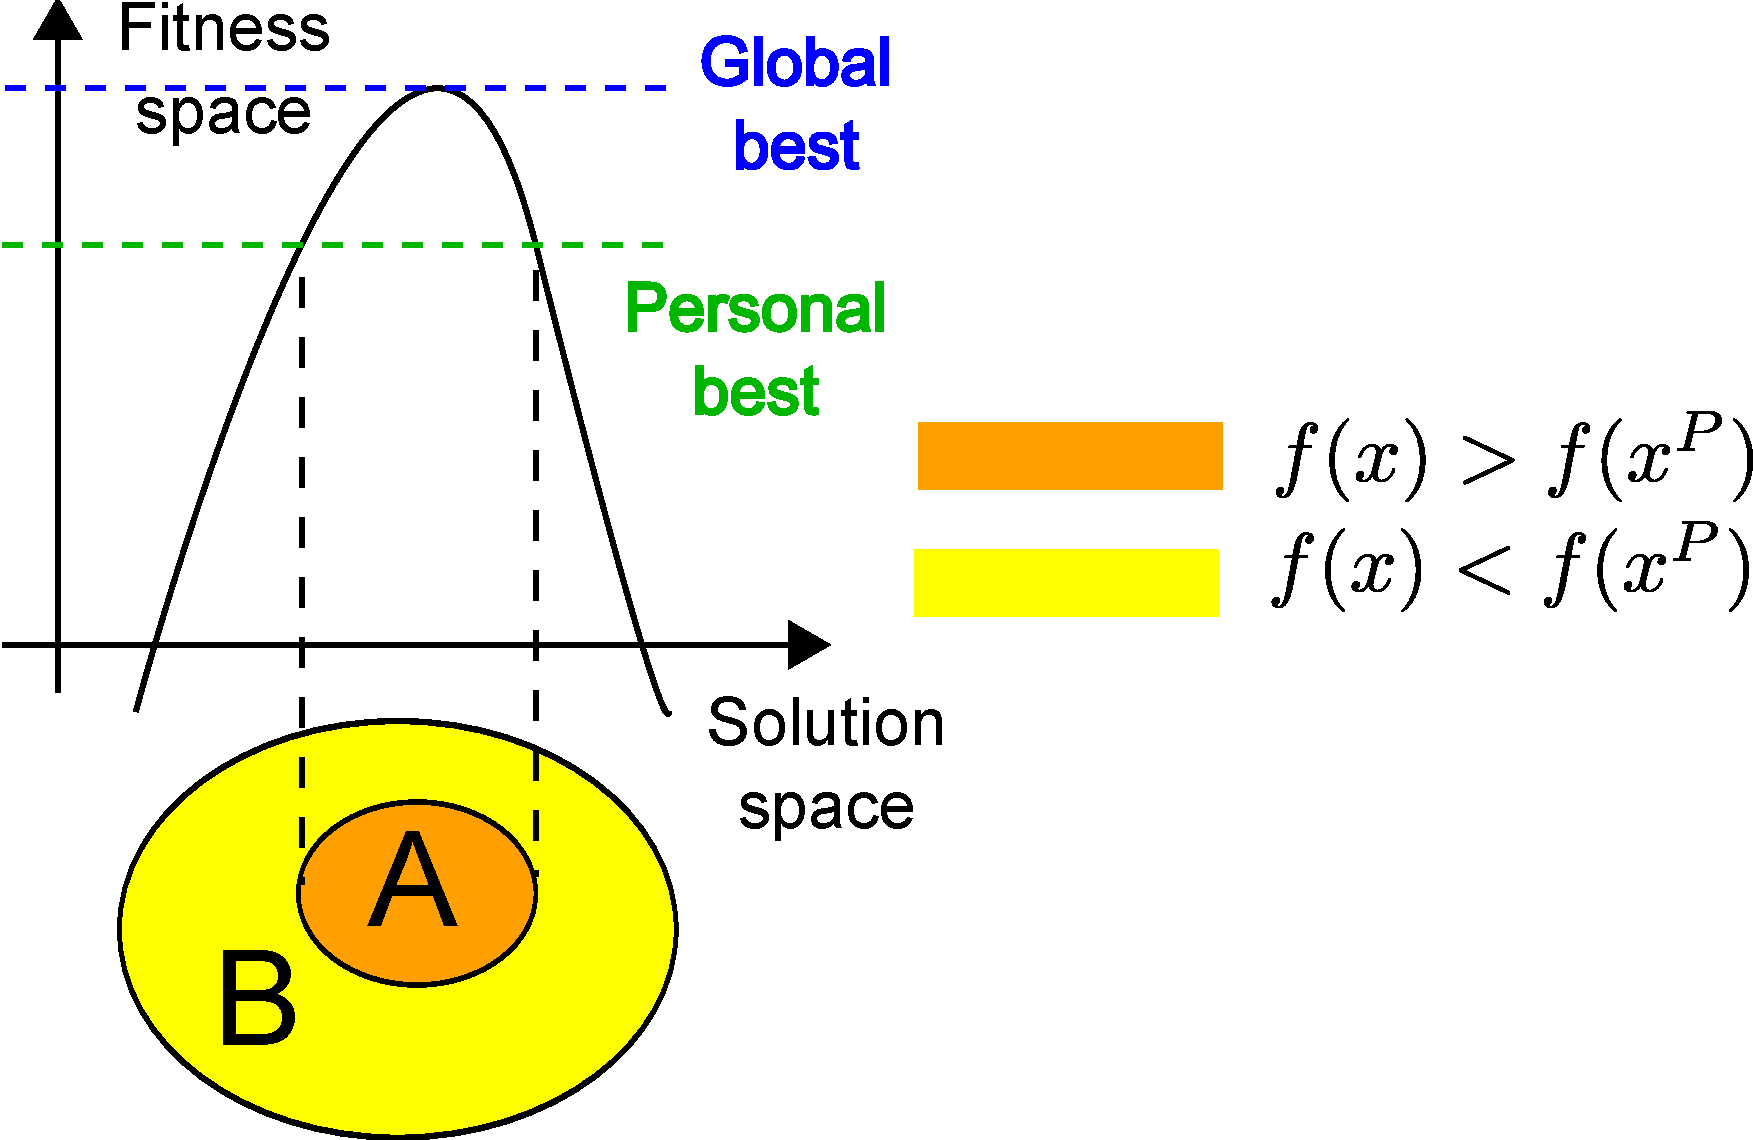
\includegraphics[width=0.7
\linewidth]{./fig/two_sets_split}
\caption{How sets $ A $ and $ B $ are defined.}
\label{fig:two_sets_split}
\end{figure}

\end{proof}
\end{mythm}

\subsubsection{ $ x^{G} \not = x^{*}  $ }

When the global best is not yet the optimal solution, the convergence of the particle will be harder to evaluate.
If  $ f(x^{*}) - \alpha_{2} ( |x| ) <  f(x) < f(x^{*}) - \alpha_{1} ( |x| ) $ is still satisfied, we can similarly have the result in Theorem \ref{thm:unimodal:particle:converge}.
Otherwise, if the particle accidentally reaches into a region that the fitness is better than the current global best, a new global best is found.
The particle might also runs stochastically in a region that the fitness is worse than both the personal best and the global best.
If the particle at least gets into a position that is better than the current personal best, the personal best will be updated. 
We notice that the particle should never stop at the current global best $ x^{G} $, which is stated in Lemma \ref{lem:unimodal:particle:nonstop}.

\begin{mylem}
\label{lem:unimodal:particle:nonstop}
In a unimodal case, if $ x^{G} \not = x^{*} $, a particle will never stop at $ x^{G} $. 
\footnote{The precision cut-off in implementation is ignored.}
\begin{proof}
Consider the velocity $ v(k+1) $ consists of two parts, inertia $ \chi v(k) $ and attractive force $ \chi \phi^{P} (x^{P}(k) - x(k) ) + \chi \phi^{G} ( x^{G} - x(k) ) $.
While the particle moves into $ x^{G} $, the attractive force becomes zero but the inertia still exists, due to the velocity moves the particle into this current position.
Thus, theoretically the particle will never stop at $ x^{G} $ when $ x^{G} \not = x^{*} $.
\end{proof} 
\end{mylem}

%\begin{mylem}
%\label{lem:unimodal:particle:input_iss2}
%In a unimodal case, when $ x^{G} \not = x^{*} $, the input-update component is input-to-state stable.
%\begin{proof}
%\end{proof}
%\end{mylem}

By Lemma \ref{lem:unimodal:particle:nonstop}, we can prove that the particle will finally get to a position that is at least better than the current global best if given enough run time in a unimodal case.
We have Theorem \ref{thm:unimodal:particle:better}.

\begin{mythm}
\label{thm:unimodal:particle:better}
In a unimodal case, when $ f( x^{G} ) < f( x^{*}) $, the particle will almost surely find a $ \hat{x^{*}} $ that $ f(\hat{x^{*}}) > f(x^{G}) $.
\begin{proof}
Because the particle cannot stop at $ x(k) = x^{G} = x^{P} $.
We will show it will finally arrives into a region that $ f(x) > f(x^{G}) $.

As in Figure \ref{fig:categorize_regions}, the solution space will be divided into three types of regions by the global best and the personal best.
\begin{itemize}
\item $ f(x) > f(x^G) $
Once a particle gets into this region, it updates both global best and personal best. 
It becomes a leader of the swarm.
\item $ f(x^{G}) > f(x) > f(x^{P}) $
Once a particle gets into this region, it updates only the personal best.
The solution space is then re-divided.
\item $ f(x) < f(x^{P}) $
When a particle is in this region, it only moves as a random walk.
\end{itemize}

\begin{figure}
\centering
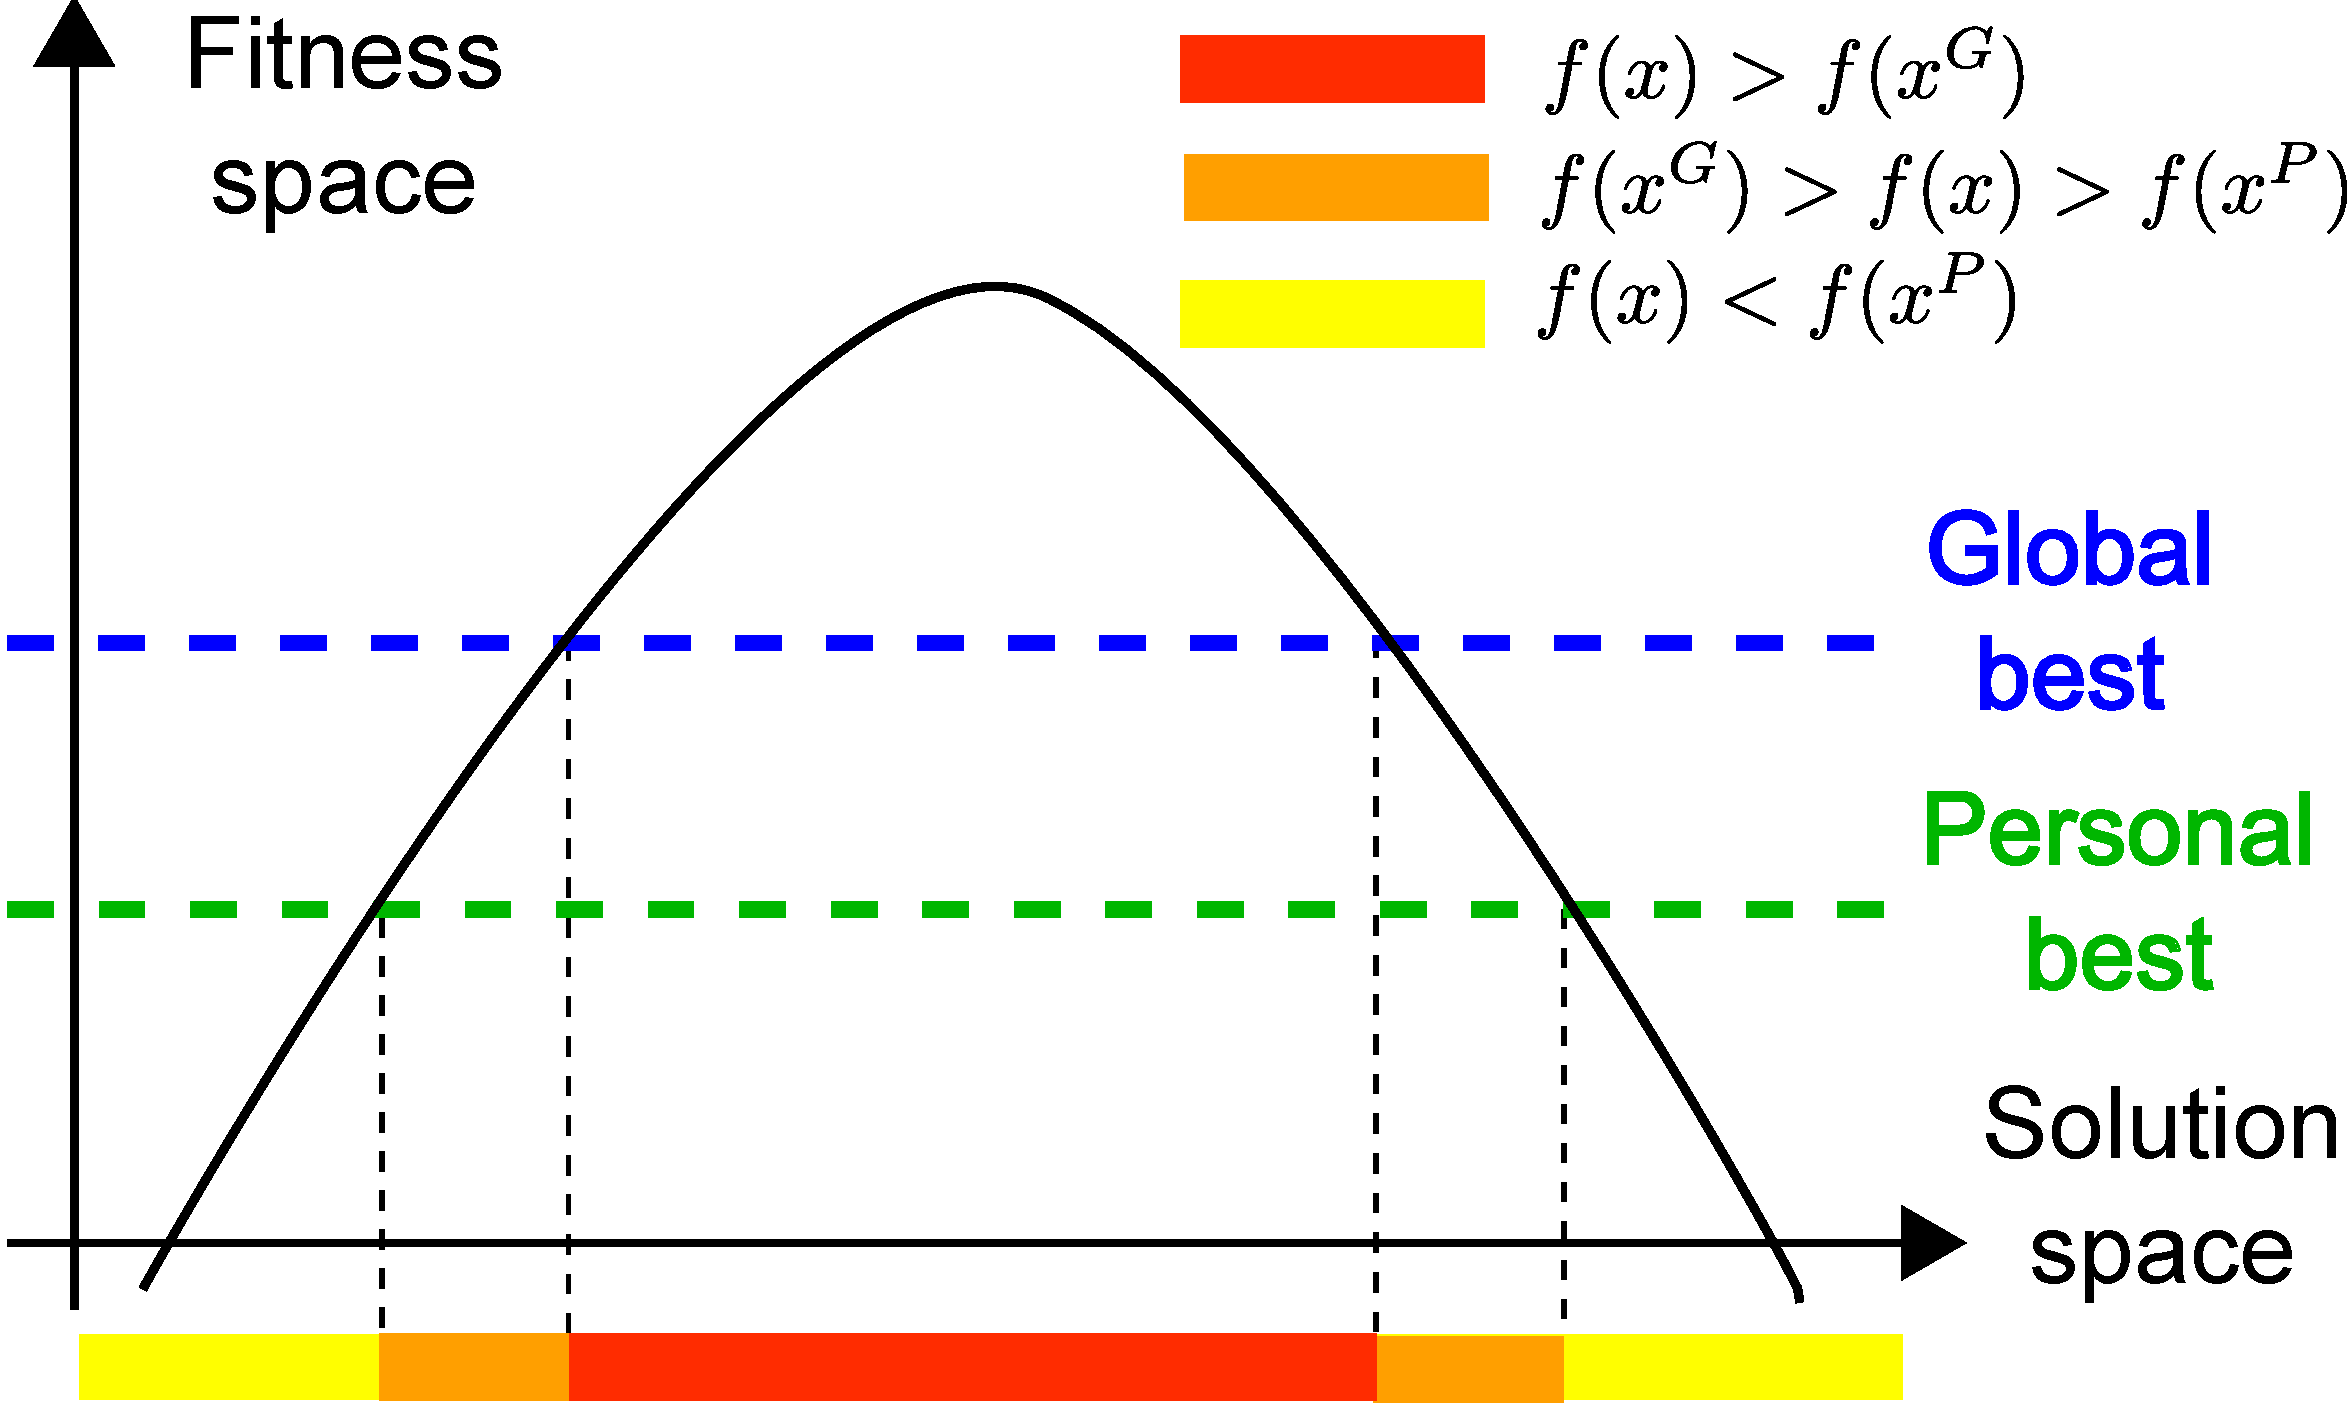
\includegraphics[width=0.7\linewidth]{./fig/categorize_regions}
\caption{How global best and personal best divide the solution space.}
\label{fig:categorize_regions}
\end{figure}

The result of the movement of a particle is determined by which region of the solution space it moves in, which forms a Markov process.
The states of the particle can be defined as
\begin{itemize}
\item \textbf{A} [$ f(x) \leq f(x^{P}) \leq f(x^{G}) $]
\item \textbf{B} [$ f(x) = f(x^{P}) \leq f(x^{G}) $] 
\item \textbf{C} [$ f(x) = f(x^{P}) \leq f(x^{G}) \land v > 0 $]
\item \textbf{D} [$ f(x) = f(x^{P}) \leq f(x^{G}) \land v = 0 $]
\item \textbf{E} [$ f(x) > f(x^{P}) = f(x^{G}) $]
\end{itemize}

The Figure \ref{fig:fsm} shows the state transitions.
When the particle is in state A, it is in random walk with attractions to the global best and personal best.
In state B, it means that the particle find a better personal best.
In state C, the particles moves into the current global best, but the velocity is not zero yet.
The only chance that the particle cannot find a better global best happens when it gets into state D.

\begin{figure}[tbph]
\centering
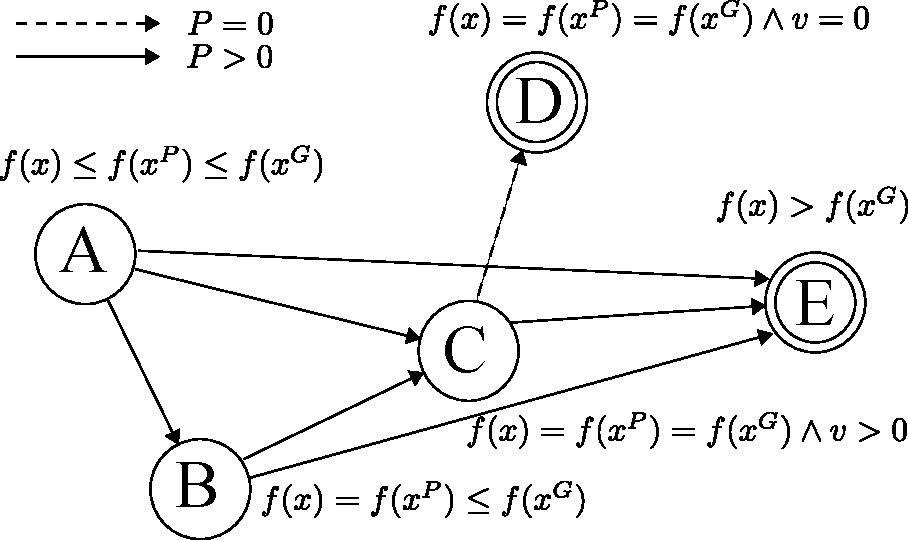
\includegraphics[width=0.7\linewidth]{./fig/fsm}
\caption{The state transition of the movement of the particle.}
\label{fig:fsm}
\end{figure}

In Figure \ref{fig:fsm}, we can see that the state will almost surely move into state E.
It means that the particle will almost surely find a better solution.
\end{proof}
\end{mythm}

\subsection{Multi-model fitness distribution}

When there are multiple modalities in the range that the particle moves, it is not easy to figure out a pattern of the behaviors that the particles share.
More factors of the fitness distribution can impact the optimal search process.
When the movement of the particle is bounded, there can be cases that the particle cannot reach the region that contains a better solution.
%[TODO: Give an example that the particle will wander between the personal best and the global best]

The exploration range is determined by the boundary of a particle's movement.
We are interested with how the particle can get closer to the optimal position $ x^{*} $.
We have Lemma \ref{lem:particle:bound_mov}.

\begin{mylem}
\label{lem:particle:bound_mov}
The bound of a particle's movement can be either 
\begin{equation}
\begin{aligned}
| x(k) - x^{*} | < \max ( \beta^{*} ( x(0) - x^{*}, k ), \\ \gamma^{*} ( \max ( | x^{G} - x^{*} | , | x^{P}(k) - x^{*}  | ) ) ),
\end{aligned}
\end{equation}
or 
\begin{equation}
| x(k) - x^{0} | < \gamma^{0} ( \max ( | x^{G} - x^{0} | , | x^{P}(k) - x^{0}  | ) ),
\end{equation}
in which $ \beta^{*} $ is $ KL $-function , $ \gamma^{*}  $ and $ \gamma^{0} () $ are $ K_{\infty} $-functions.
\begin{proof}
These can be obtained by applying $ x^{*} $ and $ x^{0} $ to Theorem \ref{thm:state_bound}.
\end{proof}
\end{mylem}
Lemma \ref{lem:particle:bound_mov} shows that the boundary of a particle's movement is determined by where the global best $ x^{G} $ and the personal best $ x^{P}(k) $ locate.

As we are interested with the probability that the particle gets into a position that is better than the current global best, we hope the distance from this position to the optimal is closer than that from the global best to the optimal.

If the boundary of the particle's movement does not contain a solution that is better than the personal best, the personal best and the global best have no chance to be updated and the particle will not be able to find a better solution.
\begin{mythm}
\label{thm:multimodal:out_of_scope}
$ \forall s \in \{ s | \, |s - x(0)| < \gamma^{0} ( \max ( | x^{G} - x^{0} | , | x^{P}(k) - x^{0}  | ) \}, f(s) < f(x^{P})  $, the probability that a particle finds a better solution is zero.
\begin{proof}
Because the particle has no chance of getting into any position that has better solution than the global best and the personal best.
Thus the boundary will also not be changed.
\end{proof}
\end{mythm}

In order to measure how likely the particle can move to a position that $ f(x) > f(x^{G}) $, we can measure the probability that $ | x(k) - x^{*} | < | x^{G} - x^{*} | $ indirectly.
We then have Corollary \ref{lem:mutimodal:particle:prob}.
\begin{mycoro}
\label{lem:mutimodal:particle:prob}
\begin{equation}
\begin{aligned}
& P( | - x^{*} | < | x^{G} - x^{*} | ) \\
& > 1 - \frac{ \gamma ( \max ( E( | x^{G} - x^{*} | ), E( | x^{P}(k) - x^{*}  | ) ) ) }{ | x^{G} - x^{*} | },
\end{aligned}
\end{equation}
in which $ \gamma () $ is a boundary function.
\begin{proof}
By Markov's inequality, we have
\begin{equation}
P( | x(k) - x^{*} | \geq | x^{G} - x^{*} | ) \leq \frac{ E( | x(k) - x^{*} | ) }{ | x^{G} - x^{*} | }.
\end{equation} 
By the mean of the position update component (details in Appendix \ref{app:mean_pso})
we can have the boundary of the mean
\begin{equation}
\label{eq:mean:opt_bound}
E( | x(k) - x^{*} | ) \leq \gamma ( \max ( E( | x^{G} - x^{*} | ), E( | x^{P}(k) - x^{*} | ) ) ),
\end{equation}
in which $ \gamma () $ is the boundary function.
\begin{equation}
\begin{aligned}
& P( | x(k) - x^{*} | < | x^{G} - x^{*} | ) \\
= & 1 - P( | x(k) - x^{*} | \geq | x^{G} - x^{*} | ) \\
> & 1 - \frac{ E( | x(k) - x^{*} | ) }{ | x^{G} - x^{*} | } \\
> & 1 - \frac{ \gamma ( \max ( E( | x^{G} - x^{*} | ) , E( | x^{P}(k) - x^{*}  | ) ) ) }{ | x^{G} - x^{*} | }.
\end{aligned}
\end{equation}
\end{proof}
\end{mycoro}

When the fitness function coarsely shows some monotonicity, we can measure the probability that the particle finds a better solution, which is given in Theorem \ref{thm:multimodal:in_scope}.

\begin{mythm}
\label{thm:multimodal:in_scope}
If the region $ R $ of $ | x - x^{*} | < \epsilon $ is monotonic, $ x(k) \in R $ and $ x^{G} \in R $, the probability that the particle find a better solution is $ P > 1 - \frac{ \gamma ( \max ( E( | x^{G} - x^{*} | ), E( | x^{P}(k) - x^{*}  | ) ) ) }{ | x^{G} - x^{*} | } $
\end{mythm} 

\subsection{Exploitation and exploration}

The property showed above provides the exploitation and exploration at a particle level.

\subsubsection{Exploitation}

The exploitation of the optimal search means the convergence property.
In a leader-follower scheme, there always exists an attraction from the global best so that the particles show convergence toward the global best.
However, the convergence property also enhance the local attraction by maintaining a personal best.
The inherent input-to-state stability guarantees that the particle could utilize the current information as the heuristic.
This makes the particle swarm optimization a convergent optimization method.

\subsubsection{Exploration}

There are also mechanisms that prevent early premature of the optimal search process, which indicates the exploration.
The import of the stochastic terms brings nondeterministic and versatile search capability, which indicates varying step length.

However, the varying step length is still limited in a range. 
There exists a boundary of the movement, as in Theorem \ref{thm:state_bound}.
This boundary implies the search capability of a particle.
As stated in Theorem \ref{thm:multimodal:out_of_scope}, the particle might not able to find a better solution and is stuck in the movement inside such a region.
Moreover, as it is shown in Lemma \ref{thm:stagnation_bound} and Lemma \ref{lem:particle:bound_mov}, the positions of the personal best and the global best can also influence the boundary of the particle's movement.
By \eqref{eq:stagnation_bound}, we can see that a bigger inconsistence between global best and personal best $ | x^{P} - x^{G} | $ usually means a bigger boundary.


%It means that a particle moves in a bounded region in the multi-modal case.
%The range of this region depends on where the global best $ x^{G} $ and the personal best $ x^{P} $ locate.
%By \eqref{eq:bound:final}, we can see that this boundary should include both the global best and the personal best.
%Particularly, the larger $ \lVert A \rVert $ is, the larger boundary is.
%It enables the explore capability of a particle.
%A smaller step provides a higher probability of finding a better solution, which locates in between the personal best and the global best.

